\documentclass{article} % For LaTeX2e
\usepackage{nips15submit_e,times}
\usepackage{hyperref}
\usepackage{url}
\usepackage{enumerate}
\usepackage{graphicx} 
\usepackage{float} 
\usepackage{subfigure} 
\usepackage{placeins}
%\documentstyle[nips14submit_09,times,art10]{article} % For LaTeX 2.09

\title{Use logistic and softmax regression to classify facial expressions on CAFE Dataset}

\author{
Shuo Xu \\
Computer Science and Engineering Department \\
UCSD \\
\texttt{s3xu@ucsd.edu} \\
\And
Changhao Shi \\
Electrical and Computer Engineering \\
UCSD \\
\texttt{cshi@ucsd.edu} \\
}

% The \author macro works with any number of authors. There are two commands
% used to separate the names and addresses of multiple authors: \And and \AND.
%
% Using \And between authors leaves it to \LaTeX{} to determine where to break
% the lines. Using \AND forces a linebreak at that point. So, if \LaTeX{}
% puts 3 of 4 authors names on the first line, and the last on the second
% line, try using \AND instead of \And before the third author name.

\newcommand{\fix}{\marginpar{FIX}}
\newcommand{\new}{\marginpar{NEW}}

\nipsfinalcopy % Uncomment for camera-ready version

\begin{document}

\maketitle

\begin{abstract}
In this report, we focuses on using logistic regression and softmax regression to classify facial expressions over CAFE dataset.
The logistic regressor is used for 2-class identification, and the softmax regressor performs identification task over 6 classes multi classification.
We performed data centralization techniques and PCA algorithm over the dataset as data pre-processing methods. We carried out a set of experiments to 
explore the effect of hyperparameters, including learning rate, the number of principle components, and contrast the ability of batch gradient descent and SGD.
In the end, we visualized the best weight vector.
\end{abstract}

\section{Introduction}

In this report, we focus on a set of classification tasks on California Facial Expresion(CAFE) dataset.
Two tasks are solved, which are

\begin{itemize}
    \item Two face classification: Use logistic regression to separate 2 kinds of facial expressions
    \item Six face classification: Use softmax regression to classify 6 emotional faces
\end{itemize}

The data pre-processing techniques we performed on the dataset are data centralization and principle component analysis.
The reason we perform such techniques comes from the fact taht centralized and decomposited data can accelerate the speed of gradient descent. 

\section{Methods}
In this section, we would show the basic pipeline of two task solutions.

\subsection{Test methods and dataset building}

In order to test the robustness of the algorithm and parameter selection, we test over all the subjects by making each one
as testee once. And report the averaged 10 accuracies over the 10 runs.

Since different task require various facial expressions, we decide to build data in a dynamical way.
This shall follow these two steps
\begin{itemize}
    \item Screen out useless data: Filter out the facial expressions labeled by 'neutral' and 'happy'.
    \item Split data: Divide the dataset in terms of 10 subjects with ratio of 80\%, 10\%, 10\% each for training, holdout and test dataset, respectively.
    \item Facial ecpression selection: Select task-related facial expressions according to the requirements
\end{itemize}

Specifically, in the second step, we iterate through all the 10 subjects and build test dataset from each subject exactly once.
The holdout dataset is selected from the rest of the subjects, and all the other 8 subjects are used as training data.

Thus, we would have 10 randomly built dataset with different testee appeared exactly once.

To be specific, for each selection of testee, the numerical features of dataset constitution should be as in Table 1.

\begin{table}[htb]
    \caption{Dataset constitution}
    \label{evaluation-of-f}
    \begin{center}
    \begin{tabular}{lll}
    \multicolumn{1}{c}{\bf Train}  &\multicolumn{1}{c}{\bf Holdout} &\multicolumn{1}{c}{\bf Test}
    \\ \hline \\
    8 subjects & 1 subject & 1 subject \\
    48 images & 6 images & 6 images \\
    \end{tabular}
    \end{center}
    \end{table}

\subsection{Data preprocessing}
After loading all the images, we carry out following pre-processing methods.
\begin{itemize}
    \item Centerize data: Calculate the mean over training dataset, and subtract this value from training, holdout and test dataset to get centerized data.
    \item PCA: Fit PCA model with centerized training data, and perform transformation(compression) over training, holdout and test dataset.
\end{itemize}

We describe some detailed implementation in PCA.

\begin{enumerate}[1]
    \item Avoid high dimentional matrix calculation
    
    By following the instruction in \href{https://stackoverflow.com/questions/13224362/principal-component-analysis-pca-in-python}{this article}, we avoided the calculation of a matrix of size 91200 by 91200 
    
    \item Each principle vector is scaled by the standard diviation.
    \item Only use the training data to compute the principle components
    
    Reason: To prevent overfitting, which means the model performs very well on training dataset but terrible on testing data. The test and validation data shouold only be used to measure the performance of the model trained on train dataset. 
    If the test or holdout dataset are exposed to PCA algorithm, the final eigen vectors would have 'learned' from test / holdout, which would cause the performance 
    to be falsely biased on validation and test dataset.
\end{enumerate}

\subsection{Two face logistic classification}
We used logistic classification over 2 sets of facial expressions.

\begin{itemize}
    \item Happy VS Maudlin
    \item Afraid VS Surprised
\end{itemize}

We performed SGD and batch gradient descent on both datasets. Here's the best parameters we used
$$learning\ rate = 0.4$$
$$epoches = 10$$

\subsection{Six face softmax classification}

We performed SGD and batch gradient descent on the dataset. Here's the parameters we used
$$learning\ rate = 0.2$$
$$epoches = 10$$

\section{Results}
In this part, we report the required results of the two tasks.

\subsection{Load and preprocess the data}

\textbf{(a) Why is it important to only use the training data to compute the principal components?}

To prevent overfitting, which means the model performs very well on training dataset but terrible on testing data. The test and validation data shouold only be used to measure the performance of the model trained on train dataset. 
If the test or holdout dataset are exposed to PCA algorithm, the final eigen vectors would have 'learned' from test / holdout, which would cause the performance 
to be falsely biased on validation and test dataset.

\textbf{(b) Six emotions}

\begin{figure}[htb]
    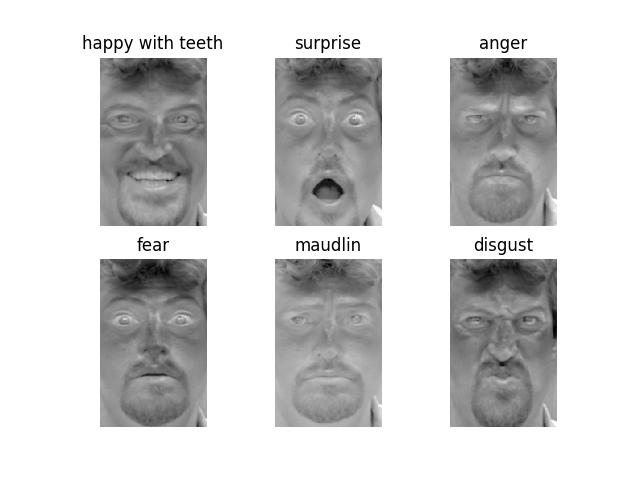
\includegraphics[width=\textwidth]{./Images/six-emotions.png}
    \caption{Six emotions}
    \label{Six emotions}
\end{figure}

\textbf{(c) First 6 eigenvectors}

\begin{figure}[htb]
    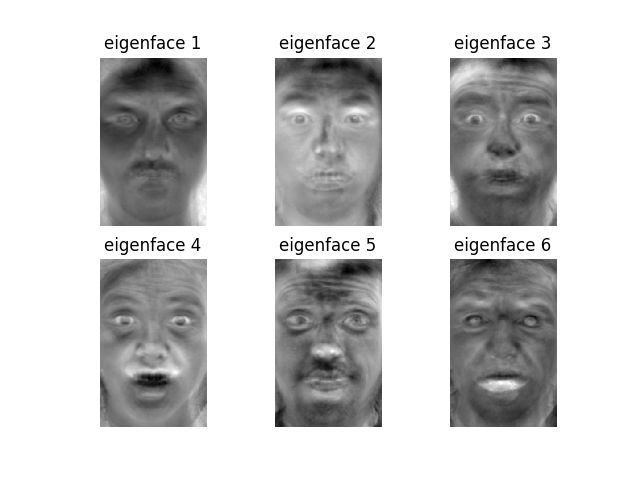
\includegraphics[width=\textwidth]{./Images/first-6-eigenvectors.png}
    \caption{First 6 eigenvectors}
    \label{First 6 eigenvectors}
\end{figure}

\newpage
\subsection{Logistic Regression}
\subsubsection{Happy vs Maudlin}

\textbf{Question: Why we only need one if we’re classifying two classes?}

Say if the probability of one class is p, the other's probability could be simply calculated as 1-p.

\textbf{Averaged error and deviation with the best learning rate}

The best learning rate we've found is \textbf{0.4} \\
Here, we display the averaged error on training and holdout dataset with deviation of epoch 2, 4, 8 and 10. Note that principle components varies.

\begin{figure}[htb]

    \centering

    \subfigure[Averaged error with 10 principle components]{
    \begin{minipage}[b]{0.5\textwidth} 
    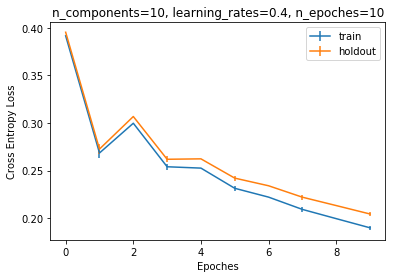
\includegraphics[width=1\textwidth]{./Images/hm-error-10-components.png} \\ 
    \end{minipage}
    }
    
    \subfigure[Averaged error with 20 principle components]{
    \begin{minipage}[b]{0.5\textwidth} 
    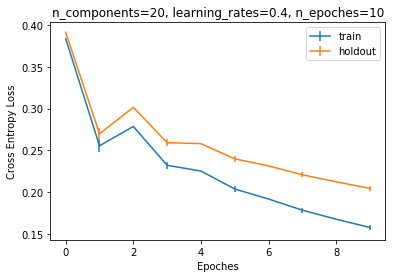
\includegraphics[width=1\textwidth]{./Images/hm-error-20-components.png} \\ 
    \end{minipage}
    }
    
    
    \subfigure[Averaged error with 40 principle components]{
    \begin{minipage}[b]{0.5\textwidth} 
    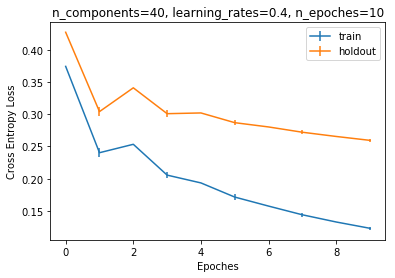
\includegraphics[width=1\textwidth]{./Images/hm-error-40-components.png} \\ 
    \end{minipage}
    }
\end{figure}

\textbf{Averaged test accuracy}

The averaged test accuracy over the 10 runs with best learning rate of 0.4 are shown as below.
\begin{itemize}
    \item number of components = 10, eccuracy = 0.955
    \item number of components = 20, eccuracy = 0.965
    \item number of components = 40, eccuracy = 0.860
\end{itemize}

\textbf{Results of various learning rate}

We've tried out 3 different learning rate in our experiments, which are \textbf{0.1, 0.4 and 0.8}. 
Here's a plot of the error of three different learning rates on the same training dataset.

\begin{figure}[htb]

    \centering
    \subfigure[Averaged error with 10 principle components]{
    \begin{minipage}[b]{0.5\textwidth} 
    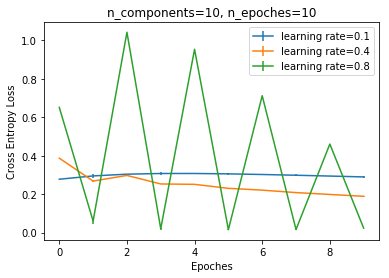
\includegraphics[width=1\textwidth]{./Images/10-components-3-learning-rate.png} \\ 
    \end{minipage}
    }
    
    \subfigure[Averaged error with 20 principle components]{
    \begin{minipage}[b]{0.5\textwidth} 
    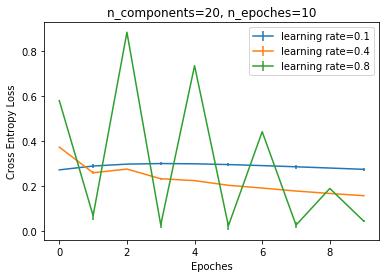
\includegraphics[width=1\textwidth]{./Images/20-components-3-learning-rate.png} \\ 
    \end{minipage}
    }
    
    
    \subfigure[Averaged error with 40 principle components]{
    \begin{minipage}[b]{0.5\textwidth} 
    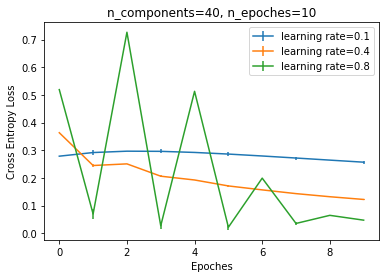
\includegraphics[width=1\textwidth]{./Images/40-components-3-learning-rate.png} \\ 
    \end{minipage}
    }
    \end{figure}

\newpage
\subsubsection{Afraid vs Surprised}

\textbf{Averaged error and deviation with the best learning rate}

The best learning rate we've found is 0.4 \\
Here, we display the averaged error on training and holdout dataset with deviation of epoch 2, 4, 8 and 10. Note that principle components varies.

\begin{figure}[htb]

    \centering

    \subfigure[Averaged error with 10 principle components]{
    \begin{minipage}[b]{0.5\textwidth} 
    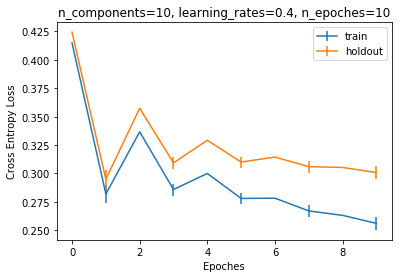
\includegraphics[width=1\textwidth]{./Images/as-error-10-components.png} \\ 
    \end{minipage}
    }
    
    \subfigure[Averaged error with 20 principle components]{
    \begin{minipage}[b]{0.5\textwidth} 
    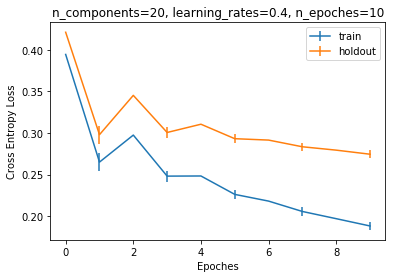
\includegraphics[width=1\textwidth]{./Images/as-error-20-components.png} \\ 
    \end{minipage}
    }
    
    
    \subfigure[Averaged error with 40 principle components]{
    \begin{minipage}[b]{0.5\textwidth} 
    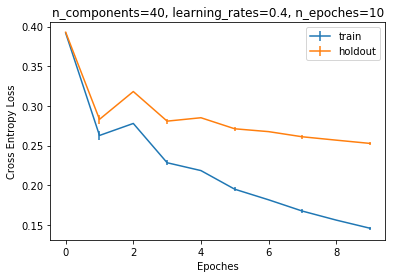
\includegraphics[width=1\textwidth]{./Images/as-error-40-components.png} \\ 
    \end{minipage}
    }
\end{figure}

\textbf{Averaged test accuracy}

The averaged test accuracy over the 10 runs with learning rate of 0.4 are shown a below.
\begin{itemize}
    \item number of components=10, accuracy = 0.690
    \item number of components=20, accuracy = 0.755
    \item number of components=40, accuracy = 0.640
\end{itemize}

\textbf{Comparison with Happy VS Maudlin}

\subsection{Softmax Regression}

\subsubsection{Evaluation on all six emotions}

\textbf{Question: What do you think would happen if we used all of the happy faces?}
The accuracy will be impaired. Because it's hard to discriminate between happy face and happy face with teeth??

\textbf{Averaged error and deviation with the best learning rate}

The best learning rate we've found is \textbf{0.2} \\
Here, we display the averaged error on training and holdout dataset. Note that principle components varies.


\begin{figure}[htb]

    \centering

    \subfigure[Averaged error with 10 principle components]{
    \begin{minipage}[b]{0.5\textwidth} 
    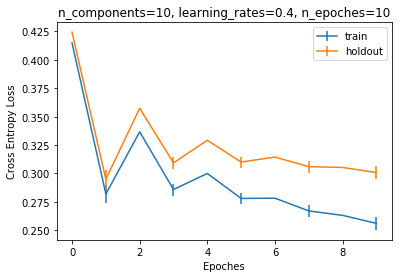
\includegraphics[width=1\textwidth]{./Images/as-error-10-components.png} \\ 
    \end{minipage}
    }
    
    \subfigure[Averaged error with 20 principle components]{
    \begin{minipage}[b]{0.5\textwidth} 
    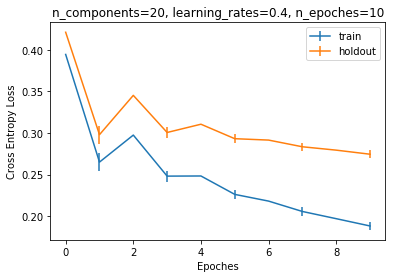
\includegraphics[width=1\textwidth]{./Images/as-error-20-components.png} \\ 
    \end{minipage}
    }
    
    
    \subfigure[Averaged error with 40 principle components]{
    \begin{minipage}[b]{0.5\textwidth} 
    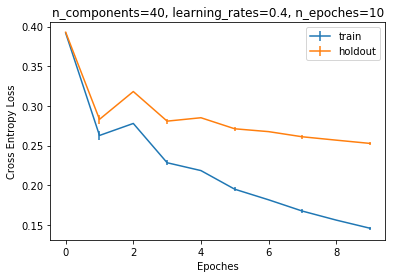
\includegraphics[width=1\textwidth]{./Images/as-error-40-components.png} \\ 
    \end{minipage}
    }
\end{figure}

\textbf{Averaged test accuracy}
In this part, we performed the softmax regression over dataset when learning rate = 0.2. 
And the results are shown as below.

\begin{figure}[htb]

    \centering

    \subfigure[Averaged error with 10 principle components]{
    \begin{minipage}[b]{0.5\textwidth} 
    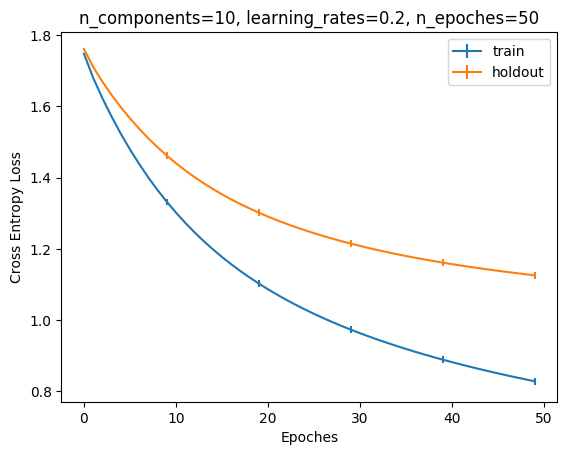
\includegraphics[width=1\textwidth]{./Images/softmax-error-10-components.png} \\ 
    \end{minipage}
    }
    
    \subfigure[Averaged error with 20 principle components]{
    \begin{minipage}[b]{0.5\textwidth} 
    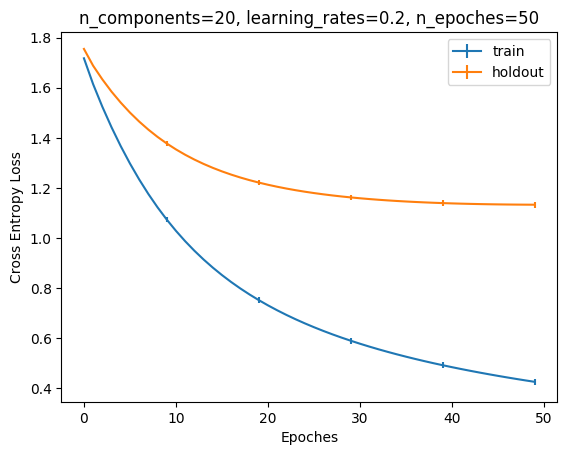
\includegraphics[width=1\textwidth]{./Images/softmax-error-20-components.png} \\ 
    \end{minipage}
    }
    
    
    \subfigure[Averaged error with 40 principle components]{
    \begin{minipage}[b]{0.5\textwidth} 
    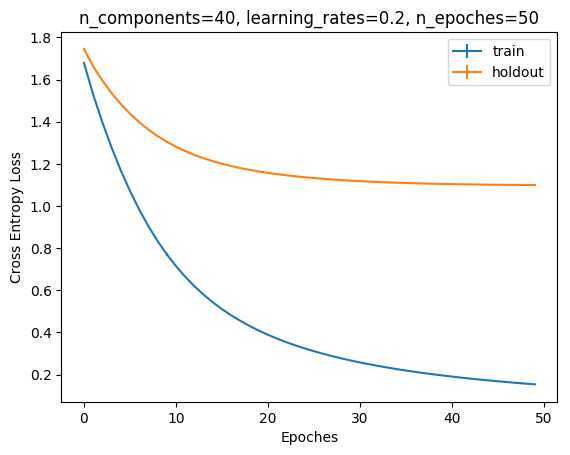
\includegraphics[width=1\textwidth]{./Images/softmax-error-40-components.png} \\ 
    \end{minipage}
    }
\end{figure}

% \begin{figure}[htb]
%     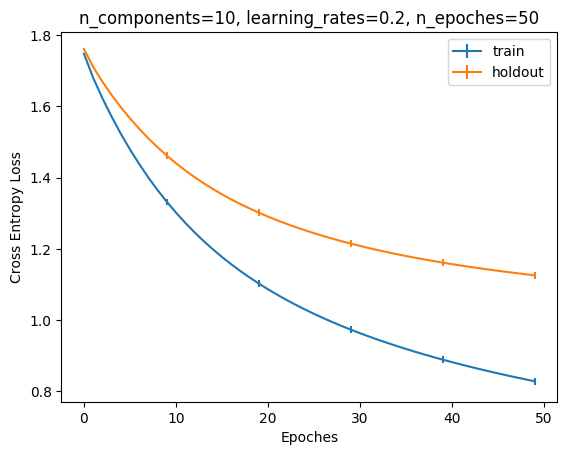
\includegraphics[width=\textwidth]{./Images/softmax-error-10-components.png}
%     \caption{Averaged error with 10 principle components}
% \end{figure}

% \begin{figure}[htb]
%     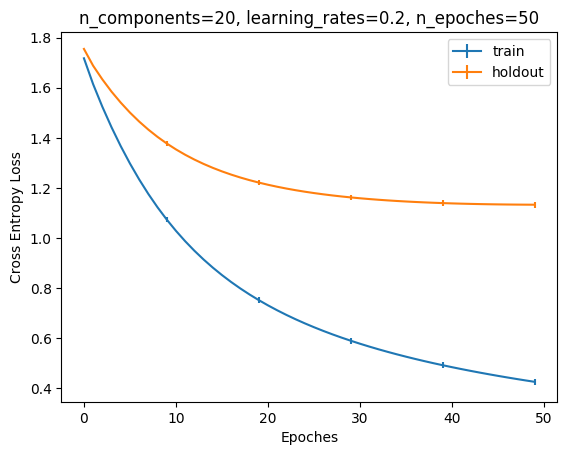
\includegraphics[width=\textwidth]{./Images/softmax-error-20-components.png}
%     \caption{Averaged error with 20 principle components}
% \end{figure}

% \begin{figure}[htb]
%     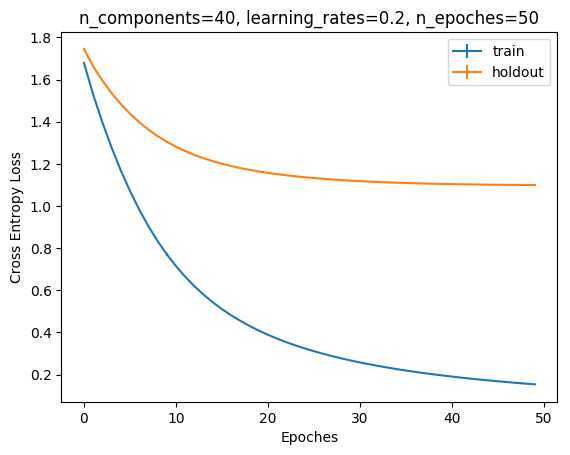
\includegraphics[width=\textwidth]{./Images/softmax-error-40-components.png}
%     \caption{Averaged error with 40 principle components}
% \end{figure}

\begin{itemize}
    \item number of components=10, accuracy = 0.607
    \item number of components=20, accuracy = 0.523
    \item number of components=40, accuracy = 0.592
\end{itemize}

\newpage
\textbf{Confusion Matrix}

In this section, we display the confusion matrix on test dataest with the selection of different components numbers.

\begin{table}[htb]
    \caption{number of principle components is 10, learning rate is 0.5, epoche is 50}
    \begin{center}
    \begin{tabular}{|c|c|c|c|c|c|c|}
     \hline
     & anger & fear & happy with teeth & disgust & surprise & maudlin \\
     \hline
     anger & 0.4 & 0.01 & 0.04 & 0.23 & 0.0 & 0.32\\
     \hline
     fear & 0.04 & 0.37 & 0.07 & 0.12 & 0.27 & 0.13\\
     \hline
     happy with teeth & 0.0 & 0.02 & 0.72 & 0.26 & 0.0 & 0.0\\
     \hline
     disgust & 0.12 & 0.05 & 0.24 & 0.5 & 0.0 & 0.09\\
     \hline
     surprise & 0.01 & 0.25 & 0.0 & 0.02 & 0.68 & 0.04\\
     \hline
     maudlin & 0.29 & 0.11 & 0.0 & 0.13 & 0.11 & 0.36\\
    \hline
    \end{tabular}
    \end{center}
\end{table}

\begin{table}[htb]
    \caption{number of principle components is 20, learning rate is 0.5, epoche is 50}
    \begin{center}
    \begin{tabular}{|c|c|c|c|c|c|c|}
    \hline
    & anger & fear & happy with teeth & disgust & surprise & maudlin \\
    \hline
    anger & 0.32 & 0.03 & 0.03 & 0.17 & 0.0 & 0.45\\
    \hline
    fear & 0.07 & 0.41 & 0.1 & 0.01 & 0.2 & 0.21\\
    \hline
    happy with teeth & 0.0 & 0.1 & 0.77 & 0.12 & 0.0 & 0.01\\
    \hline
    disgust & 0.03 & 0.09 & 0.24 & 0.49 & 0.0 & 0.15\\
    \hline
    surprise & 0.02 & 0.14 & 0.0 & 0.04 & 0.64 & 0.16\\
    \hline
    maudlin & 0.29 & 0.12 & 0.0 & 0.2 & 0.05 & 0.34\\
    \hline
    \end{tabular}
    \end{center}
\end{table}

\begin{table}[htb]
    \caption{number of principle components is 40, learning rate is 0.5, epoche is 50}
    \begin{center}
    \begin{tabular}{|c|c|c|c|c|c|c|}
    \hline
    & fear & anger & disgust & maudlin & happy with teeth & surprise \\
    % softmax confusion, n_components=[35, 40, 45], learning_rates=0.2, n_epoches=50
    \hline
    fear & 0.49 & 0.02 & 0.01 & 0.1 & 0.13 & 0.25\\
    \hline
    anger & 0.01 & 0.65 & 0.16 & 0.18 & 0.0 & 0.0\\
    \hline
    disgust & 0.14 & 0.13 & 0.56 & 0.03 & 0.14 & 0.0\\
    \hline
    maudlin & 0.14 & 0.37 & 0.13 & 0.27 & 0.0 & 0.09\\
    \hline
    happy with teeth & 0.12 & 0.0 & 0.04 & 0.0 & 0.84 & 0.0\\
    \hline
    surprise & 0.26 & 0.0 & 0.0 & 0.09 & 0.0 & 0.65\\
    \hline
    \end{tabular}
    \end{center}
\end{table}

\newpage
\FloatBarrier
\textbf{Batch VS SGD}

Here, we show the plot of error over training dataset using batch gradient and SGD.

\begin{figure}[htb]

    \centering

    \subfigure[Averaged error with 10 principle components]{
    \begin{minipage}[b]{0.5\textwidth} 
    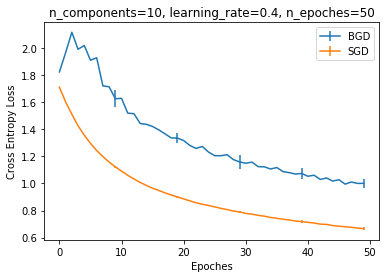
\includegraphics[width=1\textwidth]{./Images/softmax-batch-sgd-10-components.png} \\ 
    \end{minipage}
    }
    
    \subfigure[Averaged error with 20 principle components]{
    \begin{minipage}[b]{0.5\textwidth} 
    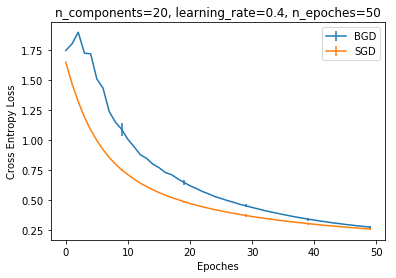
\includegraphics[width=1\textwidth]{./Images/softmax-batch-sgd-20-components.png} \\ 
    \end{minipage}
    }
    
    \subfigure[Averaged error with 40 principle components]{
    \begin{minipage}[b]{0.5\textwidth} 
    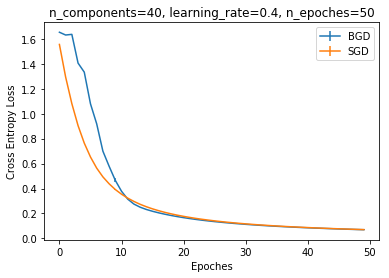
\includegraphics[width=1\textwidth]{./Images/softmax-batch-sgd-40-components.png} \\ 
    \end{minipage}
    }
\end{figure}

\FloatBarrier
\newpage
\textbf{Visualize the weight}
\begin{figure}[htb]
    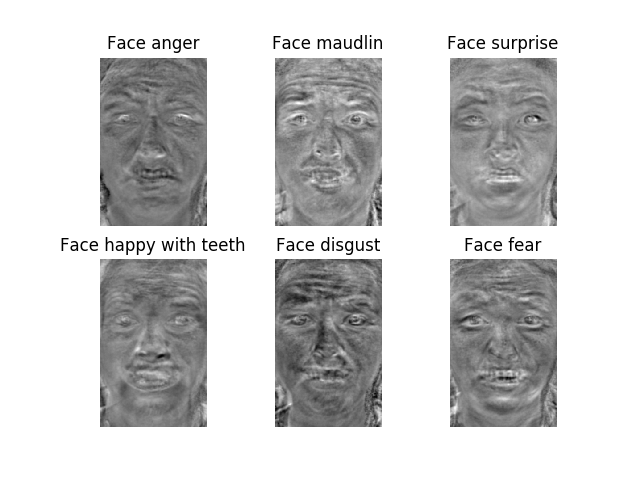
\includegraphics[width=\textwidth]{./Images/weight-visualization.png}
    \caption{Visualized weight}
\end{figure}

\subsection{Conclusion} 

In this assignment, we explore the influences of different hyperparameter on the emotion detection performance of logistic regression and softmax regression, for binary and multi-classes emotion classification tasks respectively. We first extract the eigenfaces, the principle components of face, from original images. We then train our networks, using thess new features, on the training set ,select the best network parameter (the weight of network) based on the loss of holdout set, and perform classification on the testing set to observe the network performance. We change the hyperparameter in of the network, including the number of eigenfaces, learning rates and batch size, and observe their influence on the performance of our network. 

With the number of eigenfaces, we find that the cross entropy loss on the train set and holdout set goes down with the increasing of that number. However this does not always lead to the increase of classification accuracy on the test set. An interesting finding is that, with the number of eigenfaces increasing, the classification accuracy first goes down then goes up. This suggest that the number of features is not a determinant factor for classification performance. 

With the learning rates, we find that there exist some "right" learning rate for specific problems. When the learning rate is low, the loss on the train set and holdout set normally decrease in a slow way, which makes the loss hard to converge within a limit number of epoches. In this scenario, increase of learning rate can lead to a faster convergence of loss function on the train set. However, when learning rate is over a threshold, we observe an oscillation of loss on both train set and holdout set. This phenomenon illustrates that gradient descent steps over the local minimum. With that being said, the loss function can still converge if the learning rate is not too large.

With the batch size, we compare the network performance of softmax regression of full batch gradient descent and stochastic gradient descent. The results illustrate that the stochastic gradient descent can leads to a faster convergence, compared to the batch gradient descent. This is reasonable because the stochastic gradient descent compute the gradient only on one sample each time and thus the network weight can decrease faster.

Overall, logistic regression has a satisfying performance on the binary classification task between "Happy with teeth" faces and "Maudlin" faces. We can reach a 100$\%$ accuracy on test set which shows the strength of logistic regression on the simple tasks like this. On the other hand, softmax regression has a much lower accuracy on test set. This is because the multi-classification problem on six different labels is a much difficult problem compared to a binary classification task, while softmax regression is merely a generalization of logistic regression on multi-class problem. To achieve better performance, more powerful classifier might be necessary, like multi-layer neural network.


\newpage
\subsection{Individual Contribution}

\textbf{Declaration} \\
For the coding part, we \href{https://en.wikipedia.org/wiki/Pair_programming}{pair programmed}. 
To be specific, we take turns to perform the role of driver and navigator. So almost every line of the code are 
co-authored by Shuo and Changhao.

\textbf{Shuo Xu}
\begin{itemize}
    \item Co-designed classes and the structure of the project and implemented it with Changhao
    \item Wrote up the report
    \item Participated in the mathematical formula deduction
\end{itemize}

\textbf{Changhao Shi}
\begin{itemize}
    \item Co-designed classes and the structure of the project and implemented it with Shuo
    \item Wrote up the report
    \item Participated in the mathematical formula deduction
\end{itemize}

\end{document}
